% thesis.tex
%
% Enjoy, evolve, and share!
%
% Compile it as follows:
% xelatex demo.tex
% bibtex demo.aux
% xelatex demo.tex && xelatex demo.tex
%
% Alternatively, compile it using `make -i' (see the provided Makefile).
%
% Check file `dimscthesis.cls' for other configuration options.
%
%
% This documentclass supports the following options:
% en
% 		If present, the document adds some English pages in the front matter
% 		plus changes some headings to English. Use this option if thesis is in English.
%       Omit if written in Greek.
%
% inscr
% 		If present, then a page with the inscription provided via the command
% 		\inscription{} is printed.
%
% ack
%		If present, then a page with the acknowledgements provided via the
%		command \acksEn{} is printed.
%
% preface
%		If present, then a preface page is included just before the
%		introductory chapter. The content of this page is controled via the
%		command \preface{}.
%
% oneside
%		If present, the thesis is formatted as if it will be printed on
%		only one side of each page, the other side being left blank.
%		Default is "twoside", which is used when this option is omitted.
%
\documentclass[inscr,ack,preface]{dimscthesis}

% Scans for figures relative to this file
\graphicspath{ {./figures/} }

%%%%%%%%%%%%%%%%%%%%%%%%%%%%%%%%%%%%%%%%%%%%%%%%%%%%%%%%%%%%%%%%%%%%%%%%%%%%%%%
%%%%%%%%%%%%%%%%%%%% User-specific package inclusions %%%%%%%%%%%%%%%%%%%%%%%%%
%%%%%%%%%%%%%%%%%%%%%%%%%%%%%%%%%%%%%%%%%%%%%%%%%%%%%%%%%%%%%%%%%%%%%%%%%%%%%%%
\hypersetup{
    unicode=true,                     % non-Latin characters in bookmarks
    pdffitwindow=true,                % page fit to window when opened
    pdfnewwindow=true,                % links in new window
    pdfkeywords={list, of, keyword},  % list of keywords
    colorlinks=true,                  % false: boxed links; true: colored links
    linkcolor=black,                  % color of internal links
    citecolor=black,                  % color of links to bibliography
    filecolor=black,                  % color of file links
    urlcolor=black,                   % color of external links
    pdftitle={Thesis title},          % title
    pdfauthor={Laertis Moustakas},    % author
    pdfsubject={Thesis}               % subject of the document
}
\urlstyle{same}
%%%%%%%%%%%%%%%%%%%%%%%%%%%%%%%%%%%%%%%%%%%%%%%%%%%%%%%%%%%%%%%%%%%%%%%%%%%%%%%
%%%%%%%%%%%%%%%%%%%% User-specific package inclusions %%%%%%%%%%%%%%%%%%%%%%%%%
%%%%%%%%%%%%%%%%%%%%%%%%%%%%%%%%%%%%%%%%%%%%%%%%%%%%%%%%%%%%%%%%%%%%%%%%%%%%%%%
\usepackage[shortlabels]{enumitem}
\usepackage{lscape}
\usepackage{subcaption}
\usepackage{listings}

%%%%%%%%%%%%%%%%%%%%%%%%%%%%%%%%%%%%%%%%%%%%%%%%%%%%%%%%%%%%%%%%%%%%%%%%%%%%%%%
%%%%%%%%%%%%%%%%%%%%%% User-specific configuration %%%%%%%%%%%%%%%%%%%%%%%%%%%%
%%%%%%%%%%%%%%%%%%%%%%%%%%%%%%%%%%%%%%%%%%%%%%%%%%%%%%%%%%%%%%%%%%%%%%%%%%%%%%%

%%%%%%%%%%%%%%%%%%%%%%%%%%%%%%%%%%%%%%%%%%%%%%%%%%%%%%%%%%%%%%%%%%%%%%%%%%%%%%%
%%%%%%%%%%%%%%%%%%%%%%%%%%% Required Metadata %%%%%%%%%%%%%%%%%%%%%%%%%%%%%%%%%
%%%%%%%%%%%%%%%%%%%%%%%%%%%%%%%%%%%%%%%%%%%%%%%%%%%%%%%%%%%%%%%%%%%%%%%%%%%%%%%
%
% First name, last name
%
\authorFirstGr{Όνομα}
\authorFirstAbrGr{Ο.} % abbreviation of first name
\authorMiddleGr{Μ.}   % abbreviation of father's first name
\authorLastGr{Επώνυμο}
\authorFirstEn{First}
\authorFirstAbrEn{F.}
\authorMiddleEn{M.}
\authorLastEn{Last}
\authorSN{DSXXXXXXX}

%
% Program (greek and english)
%
\programGr{ΤΙΤΛΟΣ ΠΡΟΓΡΑΜΜΑΤΟΣ ΜΕΤΑΠΤΥΧΙΑΚΩΝ ΣΠΟΥΔΩΝ}
\programEn{POSTGRADUATE MASTERS PROGRAM TITLE}

%
% The title of the thesis
%
\titleGr{Τίτλος Διπλωματικής Εργασίας}
\titleEn{Postgraduate Thesis Title}

%
% Month followed by Year
%
\dateGr{ΑΥΓΟΥΣΤΟΣ 2023}
\dateEn{AUGUST 2023}

%
% Advisor info
%
\advisorGr{Επιβλέπων Πρώτος}
\advisorRankGr{Καθηγητής}
\advisorOrgGr{ΕΚΠΑ}
\advisorEn{Board First}
\advisorRankEn{Professor}
\advisorOrgEn{NKUA}

%
% Members of the advisory board
% (the first one, will be automatically taken up by the advisor)
%
\boardTwoGr{Επιβλέπων Δεύτερος}
\boardTwoRankGr{Καθηγητής}
\boardTwoOrgGr{ΕΚΠΑ}
\boardTwoEn{Board Second}
\boardTwoRankEn{Professor}
\boardTwoOrgEn{NKUA}

\boardThreeGr{Επιβλέπων Τρίτος}
\boardThreeRankGr{Καθηγητής}
\boardThreeOrgGr{ΕΚΠΑ}
\boardThreeEn{Board Third}
\boardThreeRankEn{Professor}
\boardThreeOrgEn{NKUA}

%
% The examination date of the thesis
%
\examinationDateGr{1 Αυγούστου 2023}
\examinationDateEn{August 1, 2023}

%
% Supervisors[heading(optional, defaluts to ΕΠΙΒΛΕΠΩΝ/SUPERVISOR)]{people} (greek and english)
%
\supervisorsGr[Επιβλέποντες]{
    {\bfseries Επιβλέπων Πρώτος}, Καθηγητής ΕΚΠΑ\\
    {\bfseries Επιβλέπων Δεύτερος}, Καθηγητής ΕΚΠΑ
}
\supervisorsEn[Supervisors]{
    {\bfseries Board First}, Professor NKUA\\
    {\bfseries Board Second}, Professor NKUA
}

%
% Abstract in Greek
%
\abstractGr{%
    Η περίληψη περιλαμβάνει το σκοπό-αντικείµενο της εργασίας, τη μεθοδολογία, τα κύρια βήματα που ακολουθήθηκαν και τέλος τα κύρια αποτελέσματα.
    Μετά το τέλος της περίληψης δηλώνεται η επιστημονική περιοχή της εργασίας και 5 λέξεις κλειδιά.
    Η συνολική έκταση της περίληψης και των λέξεων δήλωσης επιστημονικής περιοχής και λέξεων-κλειδιών θα είναι 1-2 σελίδες.
}
%
% Subject area and keywords in Greek
%
\subjectAreaGr{Πρότυπο διπλωματικής σε \LaTeX{}}
\keywordsGr{λίστα, λέξεων-κλειδιών}

\abstractEn{%
    The abstract details the scope and purpose of this thesis, methodology, any experiments and the results thereof.
    You also need to declare the subject area and up to 5 keywords to be included after the abstract.
    The abstract and keywords should span no more than 2 pages.
}

%
% Subject area and keywords in English
%
\subjectAreaEn{Thesis \LaTeX{} template}
\keywordsEn{list, of, keywords}

%
% Inscription page (insc)
%
\inscription{\emph{Προαιρετική αφιέρωση.\\
        Συμπεριλαμβάνεται όταν η επιλογή \emph{inscr} προστίθεται στο \textbackslash{}documentclass.}}

%
% Acknowledgment page (ack)
%
\acks{%
    Προαιρετική σελίδα που περιλαμβάνει τις ευχαριστίες. Η σελίδα αυτή εμφανίζεται όταν η επιλογή \textit{ack} συμπεριλαμβάνεται στο \textbackslash{}documentclass.
}

%
% Preface page (preface)
%
\preface{%
    Εδώ δίνετε περισσότερες μη-επιστημονικές πληροφορίες που δεν περιγράφονται στην περίληψη ή το κυρίως κείμενο.

    Η σελίδα αυτή συμπεριλαμβάνεται με την προσθήκη της επιλογής \emph{preface} στο \textbackslash{}documentclass.
}


%%%%%%%%%%%%%%%%%%%%%%%%%%%%%%%%%%%%%%%%%%%%%%%%%%%%%%%%%%%%%%%%%%%%%%%%%%%%%%%
%%%%%%%%%%%%%%%%%%%%%%%%%%%%%% Main Matter %%%%%%%%%%%%%%%%%%%%%%%%%%%%%%%%%%%%
%%%%%%%%%%%%%%%%%%%%%%%%%%%%%%%%%%%%%%%%%%%%%%%%%%%%%%%%%%%%%%%%%%%%%%%%%%%%%%%

\begin{document}

\frontmatter

\mainmatter

% add main chapters (should be given in capital letters)
\chapter{ΕΙΣΑΓΩΓΗ} \label{introduction}

\section{Μορφοποίηση κειμένου} \label{text_formatting}

Αυτό το παράδειγμα σε \LaTeX{} αποτελεί ένα πρότυπο μορφοποίησης μεταπτυχιακών διπλωματικών εργασιών.
Το παράδειγμα αυτό εστιάζει σε διπλωματικές εργασίες γραμμένες στα Ελληνικά.
Σιγουρευτείτε ότι η επιλογή \emph{en} είναι απούσα από το \verb|\documentclass| στις πρώτες γραμμές του αρχείου .tex.

Προκειμένου η γκρίζα βιβλιογραφία να είναι ομοιόμορφη στα έγγραφα της βιβλιοθήκης---συμπεριλαμβανομένου και των μεταπτυχιακών διπλωματικών εργασιών---αυτό το πρότυπο χρησιμοποιεί μορφοποίηση όπως επιβάλλεται από το Τμήμα Πληροφορικής \& Τηλεπικοινωνιών.
Οι λεπτομέρειες μορφοποίησης είναι οι εξής:

\subsection{Μέγεθος σελίδας} \label{page_size}

Το μέγεθος της σελίδας είναι \textbf{A4}.

\subsection{Εκτύπωση σελιδών} \label{printing_pages}

Τα περιθώρια της σελίδας, και η τοποθέτηση στοιχείων στην κεφαλίδα και υποσέλιδο κάθε σελίδας εξαρτάται από το αν η εκτύπωση είναι διπλής όψης, όπως σε ένα βιβλίο, ή μονής όψης.

\subsubsection{Εκτύπωση διπλής όψης} \label{two-sided_printing}

Η διάταξη εκτύπωση διπλής όψης είναι η προεπιλεγμένη σε αυτό το πρότυπο.
Σε μονές σελίδες στα δεξιά του βιβλίου, τα δεξιά περιθώρια είναι μικρότερα από τα αριστερά περιθώρια.
Σε ζυγές σελίδες στα αριστερά του βιβλίου ισχύει το αντίστροφο: τα αριστερά περιθώρια είναι μικρότερα από τα δεξιά.

Η επικεφαλίδα περιλαμβάνει τον τίτλο της εργασίας, και τοποθετείται στα αριστερά στις μονές σελίδες και στα δεξιά στις ζυγές σελίδες.
Το υποσέλιδο περιλαμβάνει τον αριθμό της σελίδας στο κέντρο όλων των σελίδων.

\subsection{Ημερομηνίες} \label{dates}

Οι ημερομηνίες στις σελίδες, όπως ο μήνας και το έτος, αναφέρονται στην ημερομηνία εξέτασης.

\subsection{Εξώφυλλο και εμπρόσθιες σελίδες} \label{cover_and_front_matter_pages}

Η μορφοποίηση είναι όπως σε αυτό το δείγμα, τα στοιχεία είναι κεντραρισμένα εκτός και αν αναφέρεται διαφορετικά, με την εξής σειρά:

\begin{enumerate}
    \item Έμβλημα της Αθηνάς: άνω-κέντρο
    \item Όνομα του πανεπιστημίου (ΕΘΝΙΚΟ ΚΑΙ ΚΑΠΟΔΙΣΤΡΙΑΚΟ ΠΑΝΕΠΙΣΤΗΜΙΟ ΑΘΗΝΩΝ): Arial, έντονα, κεφαλαία, 14στ.
    \item Όνομα σχολής (ΣΧΟΛΗ ΘΕΤΙΚΩΝ ΕΠΙΣΤΗΜΩΝ): Arial, έντονα, κεφαλαία, 12στ.
    \item Όνομα τμήματος (ΤΜΗΜΑ ΠΛΗΡΟΦΟΡΙΚΗΣ ΚΑΙ ΤΗΛΕΠΙΚΟΙΝΩΝΙΩΝ): Arial, έντονα, κεφαλαία, 12στ.
    \item Όνομα μεταπτυχιακού προγράμματος: Arial, έντονα, κεφαλαία, 12 στ.
    \item Τύπος εργασίας (ΔΙΠΛΩΜΑΤΙΚΗ ΕΡΓΑΣΙΑ): Arial, έντονα, κεφαλαία, 12στ.
    \item Τίτλος εργασίας: Arial, έντονα, 16στ.
    \item Όνομα, αρχικό γράμμα μεσαίου ονόματος, και επίθετο συγγραφέα: Arial, έντονα, 12στ.
    \item Επιβλέπων καθηγητής (ή Επιβλέποντες αν είναι περισσότεροι του ενός) σε αριστερή στοίχιση: Όνομα και επίθετο: Arial, έντονα, 12στ., Τίτλος επιβλέποντα: Arial 12στ.\\
    Αν υπάρχουν επιβλέποντες που δεν ανήκουν στο προσωπικό της σχολής, τοποθετούνται μετά το προσωπικό με τους τίτλους τους.
    \item Τόπος εκπόνησης της εργασίας (ΑΘΗΝΑ): Arial, έντονα, κεφαλαία, 12στ.
    \item Μήνας και έτος εξέτασης της εργασίας: Arial, έντονα, κεφαλαία, 12στ.
    \item Διάστιχο: 1στ.
    \item Η αρίθμηση των σελίδων ξεκινά από τον αριθμό 1 στο εξώφυλλο, αλλά δεν εκτυπώνεται στο εξώφυλλο ούτε στις αρχικές σελίδες.
    \item Η οπίσθια όψη των σελίδων αυτών παραμένει κενή.
\end{enumerate}

\subsection{1ο εσώφυλλο (Σελίδα εξεταστικής επιτροπής)} \label{second_front_matter_page}

Μορφοποιημένο όπως στο δείγμα, τα στοιχεία είναι κεντραρισμένα εκτός και αν αναφέρεται διαφορετικά, με την εξής σειρά:

\begin{enumerate}
    \item Τύπος εργασίας (ΔΙΠΛΩΜΑΤΙΚΗ ΕΡΓΑΣΙΑ): Arial, έντονα, κεφαλαία, 12στ.
    \item Τίτλος: Arial, 12στ.
    \item Όνομα \& επίθετο συγγραφέα: Arial, έντονα, 12στ.
    \item Αριθμός μητρώου συγγραφέα: Arial, κεφαλαία, 12στ.
    \item Σε αριστερή στοίχιση: Επιβλέποντας/ες και τριμελής εξεταστική επιτροπή: Arial, έντονα, κεφαλαία, 12στ.\\
    Και τα δύο περιέχουν:
    \begin{itemize}
        \item Όνομα μέλους επιτροπής, Arial, έντονα, 12στ.
        \item Τίτλος μέλους επιτροπής, Arial, έντονα, 12στ.
        \item Υπογραφές επιτροπης
    \end{itemize}
    \item Ημερομηνία εξέτασης: Arial, έντονα, 12στ.
\end{enumerate}

Η οπίσθια όψη παραμένη κενή.

\subsection{Περίληψη} \label{abstract}

Ακολουθούν δύο περιλήψεις, μία στην Ελληνική γλώσσα και μία στη Αγγλική.
Η περίληψη περιλαμβάνει το σκοπό-αντικείµενο της εργασίας, τη μεθοδολογία, τα κύρια βήματα που ακολουθήθηκαν και τέλος τα κύρια αποτελέσματα.

Το κείμενο της περίληψης ακολουθείται από τη θεματική περιοχή και έως και 5 λέξεις-κλειδιά, στην Ελληνική και Αγγλική μετά των αντίστοιχων περιλήψεων.
Κάθε περίληψη μαζί με τη θεματική περιοχή και λέξεις-κλειδιά μπορούν να είναι έως και 2 σελίδες σε έκταση.
Οι ζυγές σελίδες παραμένουν κενές αν η περίληψη έχει έκταση 1 μόνο σελίδας.

\subsection{Άλλες εμπρόσθιες σελίδες} \label{other_front_matter_pages}

Οι υπόλοιπες εμπρόσθιες σελίδες είναι οι εξής:

\begin{enumerate}
    \item Αφιέρωση.
    Προαιρετική, συμπεριλαμβάνεται με την προσθήκη του \emph{inscr} στις επιλογές του \verb|\documentclass|.
    Η οπίσθια όψη της σελίδας παραμένει κενή.
    \item Ευχαριστίες.
    Προαιρετική, συμπεριλαμβάνεται με την προσθήκη του \emph{ack} στις επιλογές του \verb|\documentclass|.
    Η οπίσθια όψη της σελίδας παραμένει κενή.
    \item Πίνακας περιεχομένων.
    Υποχρεωτική, περιλαμβάνει τα κεφάλαια, ενοτήτων και υποδιαιρέσεις αυτών, καθώς και μια λίστα από εικόνες και μια λίστα από πίνακες, αν υπάρχουν.
    \item Πρόλογος.
    Προαιρετική, συμπεριλαμβάνεται με την προσθήκη του \emph{preface} στις επιλογές του \verb|\documentclass|.
\end{enumerate}

\subsection{Αρίθμηση σελίδων} \label{page_numbering}

Η αρίθμηση των σελίδων αρχίζει από τον αριθμό 1 στο εξώφυλλο, το Ελληνικό εξώφυλλο για εργασίες στην Ελληνική, χωρίς να εκτυπώνεται.
Όταν γίνεται η εκτύπωση και στις δύο όψεις της κάθε σελίδας (προεπιλογή), οι κενές σελίδες συμπεριλαμβάνονται στο σύνολο των σελίδων, αλλά δεν περιλαμβάνουν κεφαλίδες ή υποσέλιδα, ούτε και τον αριθμό σελίδας.
Αν η εκτύπωση γίνεται μόνο στην εμπρόσθια όψη της κάθε σελίδας (με τη προσθήκη της επιλογής \emph{oneside} στο \verb|\documentclass|), μόνο οι σελίδες στη δεξιά πλευρά του βιβλίου εκτυπώνονται και τυχόν κενές σελίδες (συμπεριλαμβανομένου και αυτών στην αριστρεή πλευρά του βιβλίου) δεν προσμετρώνται στο σύνολο των σελίδων.
Η αρίθμηση τελειώνει πάντα με την τελευταία εκτυπωμένη σελίδα.

Σε εκτυπώσεις διπλής όψης, οι αριθμοί εκτυπώνονται στη μέση κάθε υποσέλιδου.
Σε εκτυπώσεις μονής όψης, οι αριθμοί εκτυπώνονται στη δεξιά πλευρά κάθε υποσέλιδου.

\subsection{Μορφοποίηση σελίδων} \label{page_formatting}

Οι σελίδες μορφοποιούνται ως εξής:

\begin{itemize}
    \item \textbf{Περιθώρια:} 2εκ. σε όλες τις πλευρές, συν 0.5εκ. προς στο κέντρο του βιβλίου όπου δένονται οι σελίδες (δηλαδή, στα αριστερά για εκτυπωμένες μονές σελίδες και στα δεξιά για εκτυπωμένες ζυγές σελίδες)
    \item \textbf{Κεφαλίδα:} 1.25εκ. από την άνω άκρη της σελίδας.
    Περιλαμβάνει τον τίτλο της εργασίας, στα δεξιά στις μονές σελίδες, στα αριστερά στις ζυγές σελίδες σε εκτύπωση διπλής όψης.
    Εμφανίζεται μόνο στον κυρίως κορμό, δηλαδή όχι στο εξώφυλλο, στο εσώφυλλο, στις υπόλοιπες εμπρόσθιες σελίδες (περίληψη, αφιέρωση, περιεχόμενα, κ.ο.κ.), ή στις κενές σελίδες.
    \item \textbf{Υποσέλιδο:} 1.25εκ. από την κάτω άκρη της σελίδας.
    Περιλαμβάνει το όνομα του συγγραφέα
    \begin{itemize}
        \item στη δεξιά πλευρά σε μονές σελίδες, στην αριστερή πλευρά σε ζυγές σελίδες, αν η εκτύπωση είναι διπλής όψης.
        \item στην αριστερή πλευρά όλων των σελίδων αν η εκτύπωση είναι μονής όψης.
    \end{itemize}
    Εμφανίζεται μόνο στον κυρίως κορμό, δηλαδή όχι στο εξώφυλλο, στο εσώφυλλο, στις υπόλοιπες εμπρόσθιες σελίδες (περίληψη, αφιέρωση, περιεχόμενα, κ.ο.κ.), ή στις κενές σελίδες.
    \item \textbf{Αριθμός σελίδας:} συμπεριλαμβάνεται στο υποσέλιδο
    \begin{itemize}
        \item στο κέντρο σε εκτύπωση διπλής όψης.
        \item στα δεξιά σε εκτύπωση μονής όψης.
    \end{itemize}
    \item \textbf{Μορφοποίηση παραγράφου:}
    \begin{itemize}
        \item \textbf{Στοίχιση:} Πλήρης στοίχιση, κάθε γραμμή που δεν τελειώνει μια παράγραφο καταλαμβάνει ολόκληρο το μήκος της γραμμής με το απαραίτητο διάκενο μεταξύ λέξεων.
        \item \textbf{Διάκενο μεταξύ παραγράφων:} 0στ. για την πρώτη, 6στ. μεταξύ όλων των παραγράφων.
        \item \textbf{Διάστιχο μεταξύ γραμμών:} 1 γραμμή
    \end{itemize}
    \item \textbf{Γραμματοσειρά:} Arial, 12στ., Normal ή Regular
    \item \textbf{Αρίθμηση κεφάλαιου:} Arial, έντονα, 12στ. or 14 στ.
    \item \textbf{Τίτλος κεφάλαιου:} Arial, έντονα, κεφαλαία, 14στ., κεντραρισμένο
    \item \textbf{Τίτλος ενότητας και περαιτέρω υποδιαιρέσεων:} Arial, έντονα, 12στ.
    \item \textbf{Εικόνες:} Κάθε εικόνα πρέπει να φέρει μοναδικό αριθμό είτε ανα κεφάλαιο είτε σε ολόκληρο το έγγραφο.
    Θα πρέπει επίσης να συμπεριλαμβάνεται λεζάντα κάτω από την εικόνα όπως στο δείγμα.
    \item \textbf{Πίνακες:} Κάθε πίνακας πρέπει να φέρει μοναδικό αριθμό είτε ανα κεφάλαιο είτε σε ολόκληρο το έγγραφο.
    Θα πρέπει επίσης να συμπεριλαμβάνεται λεζάντα πάνω από τον πίνακα όπως στο δείγμα.
\end{itemize}

\section{Παράδειγμα ενότητας}

Ο τίτλος της ενότητας θα εμφανιστεί στον πίνακα περιεχομένων.

\subsection{Παράδειγμα υποενότητας}

Ο τίτλος της υποενότητας θα εμφανιστεί στον πίνακα περιεχομένων.

\subsubsection{Παράδειγμα υπουποενότητας}

Ο τίτλος της υπουποενότητας θα εμφανιστεί στον πίνακα περιεχομένων.

\paragraph{Παράδειγμα παραγράφου}

Ο τίτλος της παραγράφου δε θα εμφανιστεί στον πίνακα περιεχομένων.

\subparagraph{Παράδειγμα υποπαραγράφου}

Ο τίτλος της υποπαραγράφου δε θα εμφανιστεί στον πίνακα περιεχομένων.

\chapter{ΜΙΑ ΣΥΝΤΟΜΗ ΑΝΑΦΟΡΑ ΣΤΟ \LaTeX} \label{introduction_to_latex}

Το \LaTeX{} είναι μια γλώσσα στοιχειοθεσίας.
Οι συγγραφείς συντάσσουν ένα αρχείο \textbf{.tex} το οποίο μεταγλωττίζεται ένα εγγραφο, σε μορφή PDF σήμερα.
Αυτό το κεφάλαιο θα δώσει μια σύντομη, μη εξαντλητική αναφορά στη γλώσσα.

\section{Εγκατάσταση του \LaTeX} \label{installing_latex}

Αν χρησιμοποιείτε macOS ή Linux ως λειτουργικό σύστημα, οι πιθανότητες είναι ότι έχετε ήδη το \LaTeX{} προεγκατεστημένο.
Τα Windows δεν συμπεριλαμβάνουν το \LaTeX{} αρχικά.
Αν δεν έχετε το \LaTeX{}, εγκαταστήστε ένα από τα ακόλουθα:
\begin{itemize}
    \item TeX Live (\url{https://www.tug.org/texlive/}).
    Περιέχει μια ολοκληρωμένη εγκατάσταση του \LaTeX{} με τα περισσότερα πακέτα προεγκατεστημενα.
    Για αυτό απαιτεί μερικά GB αποθηκευτικού χώρου σε μια τυπική εγκατάσταση.
    Υποστηρίζει τα περισσότερα αν όχι όλα τα πακέτα που χρησιμοποιούνται σε αυτό το δείγμα.
    \item Το MiKTeX (\url{https://miktex.org/}) είναι μια πιο μινιμαλιστική εγκατάσταση.
    Η τυπική εγκατάσταση περιλαμβάνει μόνο τα απαραίτητα πακέτα, με την επιλογή να εγκατασταθούν και άλλα, είτε από την κονσόλα είτε αυτόματα κατά τη δημιουργία του PDF.
    Αυτό το έγγραφο χρησιμοποιεί πακέτα που δε συμπεριλαμβάνονται σε μια τυπική εγκατάσταση του MiKTeX, αλλά θα ερωτηθείτε για την εγκαταστασή τους όταν μεταγλωττίσετε το PDF την πρώτη φορά.
\end{itemize}

Και τα δύο προγράμματα μπορούν να εγκατασταθούν σε περιβάλλον Windows, macOS, ή Linux.

\section{Επεξεργασία} \label{editing}

Τα αρχεία \TeX{} επεξεργάζονται με τη χρήση απλού προγράμματος κειμένου, όπως το Notepad.
Η μεταγλώττιση σε PDF παραδοσιακά γίνεται από τη γραμμή εντολών.
Παρόλα αυτά, προτείνεται η χρήση προγράμματος επεξεργασίας αρχείων \TeX{}, που σχεδιάστηκε να επεξεργάζεται, να μεταγλωττίζει και να εμφανίζει αρχεία PDF σε ένα μόνο πρόγραμμα.

Μερικά προγράμματα σχεδιασμένα για επεξεργασία και σύνταξη αρχείων \TeX{} είναι:
\begin{itemize}
    \item \textbf{TeXworks} (\url{https://tug.org/texworks/}).
    Περιλαμβάνει πολύ βασικές λειτουργείες.
    Συμπεριλαμβάνεται με το TeX Live και το MiKTeX, οπότε δεν απαιτείται η εγκατάσταση αν οποιαδήποτε από τα δύο συστήματα είναι εγκατεστημένο.
    \item \textbf{Texmaker} (\url{https://www.xm1math.net/texmaker/}).
    Περιλαμβάνει πιο προχωρημένες λειτουργίες, όπως δομή εγγράφου, εισαγωγή συμβόλων, και άλλων εντολών \LaTeX{} που εισάγονται στο κείμενο με το πάτημα ενός κουμπιού.
    \item \textbf{TeXstudio} (\url{https://www.texstudio.org/}).
    Παρόμοιες λειτουργείες με το Texmaker.
    \item \textbf{Kile} (\url{https://kile.sourceforge.io/}).
    Δημιουργήθηκε από το KDE.
\end{itemize}

\section{Μεταγλώττιση} \label{compiling}

Πριν ξεκινήσουμε με τις εντολές, θα ήθελα να αναφέρω ότι αυτό το έγγραφο---είτε στην Ελληνική είτε στην Αγγλική γλώσσα---χρησιμοποιεί το πρόγραμμα XeLaTeX για τη μεταγλώττιση.
Αυτό συμβαίνει διότι το LaTeX χρησιμοποιεί χαρακτήρες ASCII για τη στοιχειοθεσία, ενώ το XeLaTeX χρησιμοποιεί χαρακτήρες Unicode, που περιλαμβάνει περισσότερους χαρακτήρες από το ASCII όπως τους ελληνικούς χαρακτήρες.

Η συνταγή μεταγλώττισης τυπικά περιλαμβάνει την εκτέλεση των κάτωθι εντολών:
\begin{enumerate}
    \item Εκτέλεση xelatex
    \item Εκτέλεση bibtex για τη μεταγλώττιση των βιβλιογραφικών αναφορών
    \item Εκτέλεση xelatex
    \item Εκτέλεση xelatex
\end{enumerate}

Όπως βλέπετε, η εντολή \textit{xelatex} τρέχει συνολικά 3 φορές, μια φορά πριν και δυο φορές μετά την εντολή \textit{bibtex}.
Αυτό συμβαίνει ώστε όλα τα \verb|\label| να έχουν βρεθεί και να συνδεθούν με τα \verb|\ref| τους.

\section{Μορφοποίηση} \label{formatting}

\subsection{Τα βασικά} \label{basics}

Δείτε το επόμενο απόσπασμα:

\begin{verbatim}
Αυτή είναι η πρώτη παράγραφος.
Αυτή είναι η επόμενη γραμμή,
αλλά παραμένει μέρος της πρώτης παραγράφου.

Αυτή είναι η δεύτερη παράγραφος.
Παρατηρήστε τη κενή γραμμή μεταξύ των δύο παραγράφων.
% Αυτό είναι ένα σχόλιο.
% Τα σχόλια δεν εμφανίζονται στο τελικό κείμενο.
% Τα σχόλια ξεκινούν με το σύμβολο "τοις εκατό" (%)
% και συνεχίζουν εως το τέλος της γραμμής.
\end{verbatim}

Στο \LaTeX{}, μεταγλωττίζεται ως εξής:

Αυτή είναι η πρώτη παράγραφος.
Αυτή είναι η επόμενη γραμμή, αλλά παραμένει μέρος της πρώτης παραγράφου.

Αυτή είναι η δεύτερη παράγραφος.
Παρατηρήστε τη κενή γραμμή μεταξύ των δύο παραγράφων.
% Αυτό είναι ένα σχόλιο. Τα σχόλια δεν εμφανίζονται στο τελικό κείμενο.
% Τα σχόλια ξεκινούν με το σύμβολο "τοις εκατό" (%)
% και συνεχίζουν εως το τέλος της γραμμής.

Όπως μπορούμε να δούμε, αν γράψουμε κάτι στην επόμενη γραμμή αυτή θα παραμείνει μέρος της παραγράφου.
Αλλά αν αφήσουμε μια κενή γραμμή μεταξύ κειμένων, το επόμενο μέρος του κειμένου εμφανίζεται σε νέα παράγραφο.

Μπορεί να παρατηρήσατε ότι οι γραμμές που άρχισαν με το '\%' δεν εκτυπώθηκαν.
Αυτό συμβαίνει διότι το σύμβολο \% λειτουργεί όπως το // σε γλώσσες προγραμματισμού όπως την C: αρχίζει ένα σχόλιο που επεκτείνεται έως το τέλος της γραμμής.
"Αλλά μια στιγμή", μπορείτε να πείτε, "πώς έβαλες το '\%' μόλις τώρα στο κείμενο";
Είναι απλό: Αν πληκτρολήσετε \verb|\%| στο \LaTeX{} θα εκτυπωθεί το \%.
Οι περισσότερες εντολές ξεκινούν την αντίστροφη κάθετο (\textbackslash), η οποία χρησιμοποιείται επίσης για την παράσταση ειδικών συμβόλων, όπως θα δούμε στο \ref{escaping}.

\subsection{Διαφυγή ειδικών χαρακτήρων} \label{escaping}
Ορισμένοι χαρακτήρες όπως το σύμβολο \% είναι ειδικόι χαρακτήρες, και συμπεριφέρονται διαφορετικά στο \LaTeX{} σε σύγκριση με απλά έγγραφα κειμένου.
Για παράδειγμα:
\begin{itemize}
    \item Το \textbf{\%} αρχίζει σχόλια.
    \item Το \textbf{\&} διαχωρίζει κολώνες σε στήλες ενός πίνακα.
    \item Το \textbf{\textbackslash\textbackslash} είτε δημιουργεί μια νέα γραμμή στην ίδια παράγραφο είτε μια νέα γραμμή σε έναν πίνακα.
    \item Τα \textbf{\{} και \textbf{\}} για τη δημιουργεία group.
    \item Το \textbf{\$} για τη γραφή μαθηματικών πράξεων.
    \item Τα \textbf{\# \_ \~{} \^{}} ως άλλοι ειδικοί χαρακτήρες.
\end{itemize}

Οι περισσότεροι χαρακτήρες διαφεύγουν (γράφονται δηλαδή κυριολεκτικά) πε την προσθήκη της αντίστροφης καθέτου πριν από το χαρακτήρα (π.χ. \textbackslash\&).
Αλλά για την εκτύπωση της αντίστροφης καθέτου, μόνο η εντολή \verb|\textbackslash| θα εκτυπώσει την '\textbackslash' κυριολεκτικά.

\subsection{εντολές μορφοποίησης} \label{formatting_commands}

Κάποιες εντολές της \LaTeX{} συμπεριφέρονται όπως στους επεξεργαστές κειμένου.
Για παράδειγμα:

\begin{center}
    \begin{tabular}{c|c}
        Αυτό... & θα εκτυπώσει αυτό \\
        \hline
        \verb|\textbf{έντονο}| & \textbf{έντονο} \\
        \verb|\textit{πλάγιο}| & \textit{πλάγιο} \\
        \verb|\underline{υπογραμμισμένο}| & \underline{υπογραμμισμένο} \\
        \verb|\textbf{\textit{έντονο και πλάγιο}}| & \textbf{\textit{έντονο και πλάγιο}}
    \end{tabular}
\end{center}

Θέλετε να βάλετε κάτι στο κέντρο της σελίδας όπως τον παραπάνω πίνακα;
Απλά γράψτε κάτι όπως:
\begin{verbatim}
\begin{center}
    Είμαι στο κέντρο της σελίδας!
    Ξεκινώ στο αρχείο .tex με \verb|\begin{center}|
    και τελειώνω με \verb|\end{center}|.
\end{center}
\end{verbatim}

και θα εκτυπωθεί:

\begin{center}
    Είμαι στο κέντρο της σελίδας!
    Ξεκινώ στο αρχείο .tex με \verb|\begin{center}|
    και τελειώνω με \verb|\end{center}|.
\end{center}

Θέλετε να δημιουργήσετε μια λίστα;
Για μη-ταξινομημένες λίστες (με τελείες):
\begin{verbatim}
\begin{itemize}
    \item Αυτό είναι ένα αντικείμενο σε περιβάλλον \textit{itemize}.
    \item Κάθε αντικείμενο αρχίζει με \verb|\item|
          και συνεχίζει μέχρι το επόμενο \verb|\item|
          ή το \verb|\end{itemize}|.
    \item Μπορείτε να εμφωλεύσετε λίστες.
          \begin{itemize}
              \item Αρκεί να δημιουργήσετε ένα
                    \textit{itemize} περιβάλλον εσωτερικά.
          \end{itemize}
\end{itemize}
\end{verbatim}

θα παράξει:
\begin{itemize}
    \item Αυτό είναι ένα αντικείμενο σε περιβάλλον \textit{itemize}.
    \item Κάθε αντικείμενο αρχίζει με \verb|\item|
    και συνεχίζει μέχρι το επόμενο \verb|\item|
    ή το \verb|\end{itemize}|.
    \item Μπορείτε να εμφωλεύσετε λίστες.
    \begin{itemize}
        \item Αρκεί να δημιουργήσετε ένα
        \textit{itemize} περιβάλλον εσωτερικά.
    \end{itemize}
\end{itemize}

\clearpage

Αν θέλετε να δημιουργήσετε μια ταξινομημένη λίστα, με αριθμούς:
\begin{verbatim}
\begin{enumerate}
    \item Αυτό είναι ένα αριθμημένο αντικείμενο
          σε περιβάλλον \textit{enumerate}.
    \item Συμπεριφέρεται όπως στο περιβάλλον \textit{itemize}.
          Αλλά αντί για τελείες που είναι ίδιες για κάθε αντικείμενο,
          βλέπετε μια σειρά από αριθμούς ή γράμματα.
    \item Όπως και πριν, μπορείτε να εμφωλεύσετε λίστες.
          \begin{enumerate}
              \item Κάπως έτσι.
              \item Φυσικά, μπορείτε να πάτε και πιο βαθιά:
                    \begin{itemize}
                        \item Μπορείτε ακόμη και να εμφωλεύσετε
                              μη-ταξινομημένες λίστες.
                              \begin{enumerate}
                                  \item Πόσο βαθιά μπορούμε να πάμε;
                              \end{enumerate}
                    \end{itemize}
          \end{enumerate}
    \item Επιτέλους, είμαστε πίσω!
\end{enumerate}
\end{verbatim}

this is what you get:
\begin{enumerate}
    \item Αυτό είναι ένα αριθμημένο αντικείμενο
          σε περιβάλλον \textit{enumerate}.
    \item Συμπεριφέρεται όπως στο περιβάλλον \textit{itemize}.
          Αλλά αντί για τελείες που είναι ίδιες για κάθε αντικείμενο,
          βλέπετε μια σειρά από αριθμούς ή γράμματα.
    \item Όπως και πριν, μπορείτε να εμφωλεύσετε λίστες.
          \begin{enumerate}
              \item Κάπως έτσι.
              \item Φυσικά, μπορείτε να πάτε και πιο βαθιά:
              \begin{itemize}
                  \item Μπορείτε ακόμη και να εμφωλεύσετε
                        μη-ταξινομημένες λίστες.
                  \begin{enumerate}
                      \item Πόσο βαθιά μπορούμε να πάμε;
                  \end{enumerate}
              \end{itemize}
          \end{enumerate}
    \item Επιτέλους, είμαστε πίσω!
\end{enumerate}

Για την προθήκη υποσημειώσεων, μπορείτε να γράψετε κάτι σαν αυτό:

\begin{verbatim}
Hello there!\footnote{General Kenobi!}
\end{verbatim}

για να λάβετε:

Hello there!\footnote{General Kenobi!}

Θέλετε να προσθέσετε URLs στο έγγραφο; Είναι απλό! Απλά γράψτε:

\begin{verbatim}
Αρχική σελίδα του \TeX{} Users Group: \url{https://www.tug.org/}
\end{verbatim}

για να εκτυπωθεί:

Αρχική σελίδα του \TeX{} Users Group: \url{https://www.tug.org/}

Και μιλώντας για συνδέσμους, αν θέλετε να προθέσετε μια βιβλιγραφική αναφορά όπως είναι δηλωμένη στο αρχείο \textbf{references.bib}, γράψτε:

\begin{verbatim}
Ο αλγόριθμος K-means\cite{bib:k_means_clustering_algorithm}
είναι γνωστός αλγόριθμος για clustering.
\end{verbatim}

για να μεταγλωττιστεί σε:

Ο αλγόριθμος K-means\cite{bib:k_means_clustering_algorithm}
είναι γνωστός αλγόριθμος για clustering.

Απλά δώστε προσοχή στο πώς είναι γραμμένη η ετικέτα της αναφοράς στο αρχείο \textbf{references.bib}.
Έχει δοθεί ένα δείγμα του αρχείου σε αυτό το παράδειγμα.
Οι βιβλιογραφικές αναφορές δεν είναι απαραίτητο να ξεκινούν με "bib:", απλά βοηθά στην οργάνωση των ετικετών.

Τέλος, αν επιθυμείτε να κατασκευάσετε σύνδεσμο σε άλλη αναφορά στο κείμενο, το:
\begin{verbatim}
Μεταβείτε στο κεφάλαιο \ref{figures_and_tables}.
\end{verbatim}

θα εμφανιστεί ως:

Μεταβείτε στο κεφάλαιο \ref{figures_and_tables}.

Όπως βλέπετε, αυτό όχι μόνο εμφανίζει τον αριθμό του κεφάλαιου "ΕΙΚΟΝΕΣ ΚΑΙ ΠΙΝΑΚΕΣ", αλλά κάνοντας κλικ πάνω του θα μεταβείτε στην αρχή του κεφάλαιου αυτού.
Αυτό μπορεί να χρησιμποιηθεί για να αναφερθείτε σε οτιδήποτε έχει την εντολή \verb|\label{label_key}|.
Απλά προσθέστε μια ετικέτα με \verb|\label{key}| σε ένα σημείο, και προσθέστε αναφορές (συνδέσμους) με \verb|\ref{key}|.

Οι εικόνες και οι πίνακες αναλύονται στο επόμενο κεφάλαιο.
Αν επιθυμείτε να μάθετε περισσότερο για εντολές \LaTeX{}, μπορείτε να λάβετε βοήθεια στο διαδίκτυο.

\subsection{Προσθήκη μαθηματικών εξισώσεων} \label{adding_math_equations}

Το \LaTeX{} υποστηρίζει επίσης την εισαγωγή μαθηματικών τύπων και εξισώσεων.
Αυτές οι εκφράσεις τείνουν να χρησιμοποιούν διαφορετική σύνταξη από το υπόλοιπο έγγραφο.

Υπάρχουν δύο τρόποι εισαγωγής μαθηματικών εκφράσεων: \emph{inline} και \emph{display}.

Στο inline, η μαθηματική έκφραση εκτυπώνεται στην ίδια παράγραφο με το υπόλοιπο κείμενο.
Για παράδειγμα, γράφοντας:
\begin{verbatim}
Μία από τις δημοφιλέστερες εξισώσεις του Άλμπερτ Αϊνστάιν
είναι η \(E = mc^2\),
όπου \(E\) η ενέργεια,
\(m\) η μάζα,
\(c\) η ταχύτητα του φωτός (περίπου 300000000 m/s).
\end{verbatim}

θα εκτυπωθεί:

Μία από τις δημοφιλέστερες εξισώσεις του Άλμπερτ Αϊνστάιν
είναι η \(E = mc^2\),
όπου \(E\) η ενέργεια,
\(m\) η μάζα,
\(c\) η ταχύτητα του φωτός (περίπου 300000000 m/s).

Στο display, οι μαθηματικές εκφράσεις εμφανίζονται σε δικές τους παραγράφους, συνήθως στο κέντρο της σελίδας.
Για παράδειγμα, γράφοντας:
\begin{verbatim}
Ο νόμος του Ωμ εκφράζεται ως:
\[V = I R \quad \textrm{ή} \quad
I = \frac{V}{R} \quad \textrm{ή} \quad
R = \frac{V}{I} \]
όπου \(V\) η τάση,
\(I\) η ένταση του ηλεκτρικού ρεύματος,
\(R\) η αντίσταση.
\end{verbatim}

θα εμφανιστεί:

Ο νόμος του Ωμ εκφράζεται ως:
\[V = I R \quad \textrm{ή} \quad
I = \frac{V}{R} \quad \textrm{ή} \quad
R = \frac{V}{I} \]
όπου \(V\) η τάση,
\(I\) η ένταση του ηλεκτρικού ρεύματος,
\(R\) η αντίσταση.

Και για αριθμημένες εξισώσεις:
\begin{verbatim}
Ο νόμος των αερίων εκφράζεται ως:
\begin{equation}
    p V = n R T
\end{equation}
όπου \(p\) η πίεση του αερίου,
\(V\) ο όγκος,
\(n\) ο αριθμός των mol,
\(R\) η σταθερά του αερίου,
\(T\) η θερμοκρασία σε βαθμούς Κέλβιν.
\end{verbatim}

για να εμφανιστεί:

Ο νόμος των αερίων εκφράζεται ως:
\begin{equation}
    p V = n R T
\end{equation}
όπου \(p\) η πίεση του αερίου,
\(V\) ο όγκος,
\(n\) ο αριθμός των mol,
\(R\) η σταθερά του αερίου,
\(T\) η θερμοκρασία σε βαθμούς Κέλβιν.

\chapter{ΕΙΚΟΝΕΣ ΚΑΙ ΠΙΝΑΚΕΣ} \label{figures_and_tables}

\section{Εισαγωγή πινάκων} \label{inserting_tables}

Παρακάτω είναι ένα δείγμα πίνακα με τη λεζάντα του.
Σιγουρετείτε ότι η λεζάντα βρίσκεται \textbf{πάνω} από τον πίνακα.
Για παράδειγμα, αυτός ο \LaTeX{} κώδικας:

\begin{verbatim}
\begin{table}
    % λεζάντα πριν από τον πίνακα
    \caption{Ένα δείγμα αρχείου καταγραφής,
        ταξινομημένα ανάλογα με την ημερομηνία συμβάντος}
    % αυτό εισάγει μια ετικέτα και προσθέτει τον πίνακα
    % στη λίστα των πινάκων
    \label{tbl:event_log_sample}
        \begin{center} % κεντράρισμα στη σελίδα
        \begin{tabular}{c|c|c}
            \textbf{Αριθμός περιστατικού} & \textbf{Συμβάν} &
            \textbf{Ημερομηνία \& ώρα} \\
            \hline
            1 & Συμβάν Α & 2021-05-24T12:30:00Z \\
            1 & Συμβάν Β & 2021-05-24T12:30:26Z \\
            1 & Συμβάν Γ & 2021-05-24T12:31:04Z \\
            2 & Συμβάν Α & 2021-05-24T13:19:39Z \\
            2 & Συμβάν Β & 2021-05-24T13:19:50Z \\
            3 & Συμβάν Α & 2021-05-24T13:19:59Z \\
            2 & Συμβάν Γ & 2021-05-24T13:22:14Z \\
            3 & Συμβάν Β & 2021-05-24T13:24:24Z \\
            4 & Συμβάν Α & 2021-05-24T13:25:06Z \\
            3 & Συμβάν Γ & 2021-05-24T13:25:27Z \\
            4 & Συμβάν Β & 2021-05-24T13:25:53Z \\
            4 & Συμβάν Γ & 2021-05-24T13:27:48Z \\
            \hline
        \end{tabular}
    \end{center}
\end{table}
\end{verbatim}

θα εμφανίσει τον Πίνακα \ref{tbl:event_log_sample}:

\begin{table}
    % λεζάντα πριν από τον πίνακα
    \caption{Ένα δείγμα αρχείου καταγραφής,
        ταξινομημένα ανάλογα με την ημερομηνία συμβάντος}
    % αυτό εισάγει μια ετικέτα και προσθέτει τον πίνακα
    % στη λίστα των πινάκων
    \label{tbl:event_log_sample}
    \begin{center} % κεντράρισμα στη σελίδα
        \begin{tabular}{c|c|c}
            \textbf{Αριθμός περιστατικού} & \textbf{Συμβάν} &
            \textbf{Ημερομηνία \& ώρα} \\
            \hline
            1 & Συμβάν Α & 2021-05-24T12:30:00Z \\
            1 & Συμβάν Β & 2021-05-24T12:30:26Z \\
            1 & Συμβάν Γ & 2021-05-24T12:31:04Z \\
            2 & Συμβάν Α & 2021-05-24T13:19:39Z \\
            2 & Συμβάν Β & 2021-05-24T13:19:50Z \\
            3 & Συμβάν Α & 2021-05-24T13:19:59Z \\
            2 & Συμβάν Γ & 2021-05-24T13:22:14Z \\
            3 & Συμβάν Β & 2021-05-24T13:24:24Z \\
            4 & Συμβάν Α & 2021-05-24T13:25:06Z \\
            3 & Συμβάν Γ & 2021-05-24T13:25:27Z \\
            4 & Συμβάν Β & 2021-05-24T13:25:53Z \\
            4 & Συμβάν Γ & 2021-05-24T13:27:48Z \\
            \hline
        \end{tabular}
    \end{center}
\end{table}


\pagebreak

\section{Εισαγωγή εικόνων} \label{inserting_figures}

Παρακάτω είναι ένα παράδειγμα εισαγωγής εικόνας με τη λεζάντα του.
Σιγουρευτείτε ότι η λεζάντα βρίσκεται \textbf{κάτω} από την εικόνα.
Για παράδειγμα αυτός ο κώδικας \LaTeX{}:

\begin{verbatim}
\begin{figure}
    % Προσδιορίτε την τοποθεσία του αρχείου εικόνων
    % στην εντολή \includegraphics
    % Θα πρέπει να είναι εσωτερικά σε σχέση με μία από τις τοποθεσίες
    % στην εντολή \graphicspath στις αρχικές γραμμές του αρχείου
    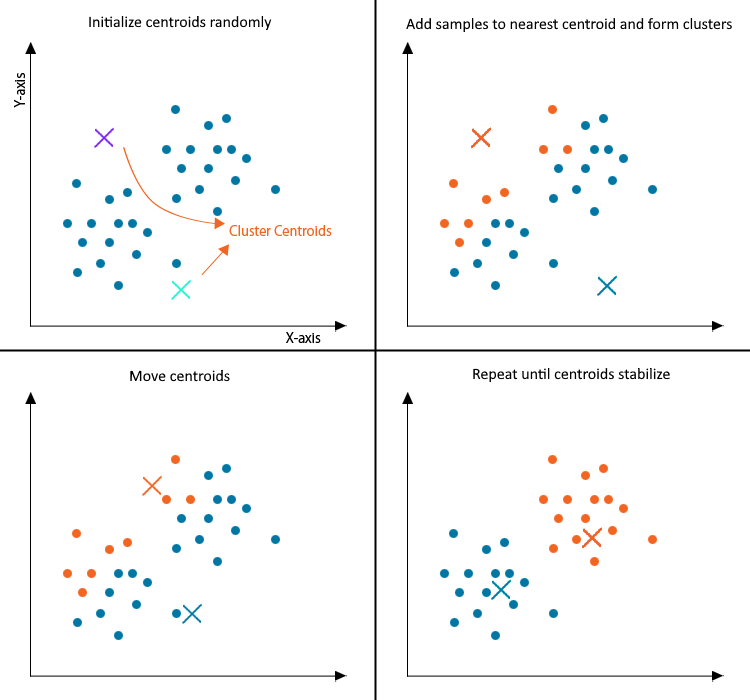
\includegraphics[width=\linewidth]{k-means_steps}
    % Τοποθέτηση λεζάντας κάτω από την εικόνα
    \caption{Τα βήματα του αλγορίθμου k-means.
        \cite{bib:k_means_clustering_algorithm}}
    % Προσθήκη ετικέτας στη λεζάντα
    % γι αν συμπεριληφθεί στον πίνακα των εικόνων
    \label{fig:k-means_steps}
\end{figure}
\end{verbatim}

θα εμφανίσει την Εικόνα \ref{fig:k-means_steps}:

\begin{figure}
    % Προσδιορίτε την τοποθεσία του αρχείου εικόνων
    % στην εντολή \includegraphics
    % Θα πρέπει να είναι εσωτερικά σε σχέση με μία από τις τοποθεσίες
    % στην εντολή \graphicspath στις αρχικές γραμμές του αρχείου
    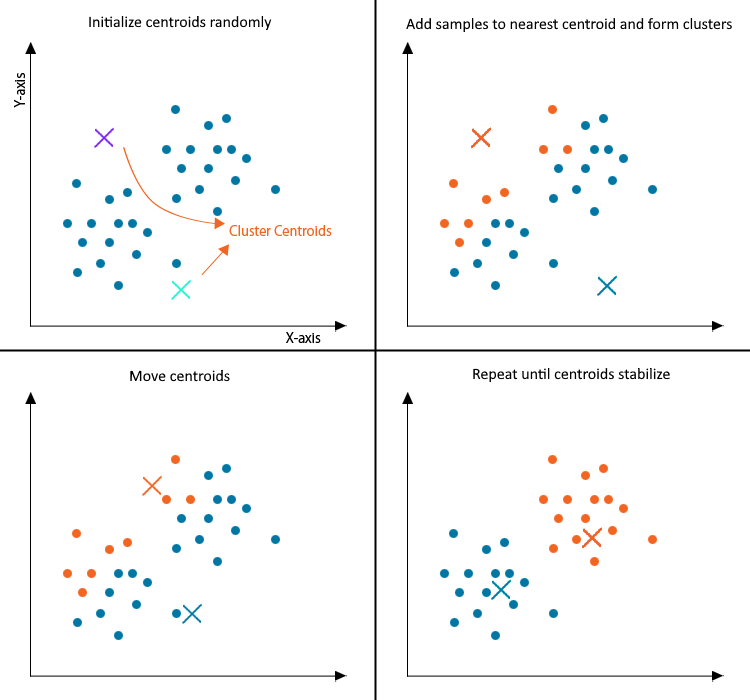
\includegraphics[width=\linewidth]{k-means_steps}
    % Τοποθέτηση λεζάντας κάτω από την εικόνα
    \caption{Τα βήματα του αλγορίθμου k-means.
        \cite{bib:k_means_clustering_algorithm}}
    % Προσθήκη ετικέτας στη λεζάντα
    % ώστε να συμπεριληφθεί στον πίνακα των εικόνων
    \label{fig:k-means_steps}
\end{figure}

\backmatter

% abbreviations table
\abbreviations
\begin{center}
    \renewcommand{\arraystretch}{1.5}
    \begin{longtable}{ l @{\qquad} l }
        \toprule
        AI    & Artificial Intelligence         \\
        SPARQL & SPARQL Protocol and RDF Query Language \\
        OWL    & Web Ontology Language                  \\
        OGC    & Open Geospatial Consortium             \\
        \bottomrule
    \end{longtable}
\end{center}

% appendix
\begin{appendix}
    % mark the beginning of the appendix
    \appendixstartedtrue

    \chapter{ΠΑΡΑΡΤΗΜΑ Α}

    \chapter{ΠΑΡΑΡΤΗΜΑ Β}

    % add appendix line to ToC
    \phantomsection
    \addcontentsline{toc}{chapter}{ΠΑΡΑΡΤΗΜΑΤΑ}
\end{appendix}

% manually include the bibliography
\bibliographystyle{IEEEtran}
{\footnotesize \bibliography{IEEEabrv,references}}
% include it also in ToC (do sth on your own)
\addcontentsline{toc}{chapter}{ΑΝΑΦΟΡΕΣ}

\end{document}
